\begin{figure}[!htb]
\centering
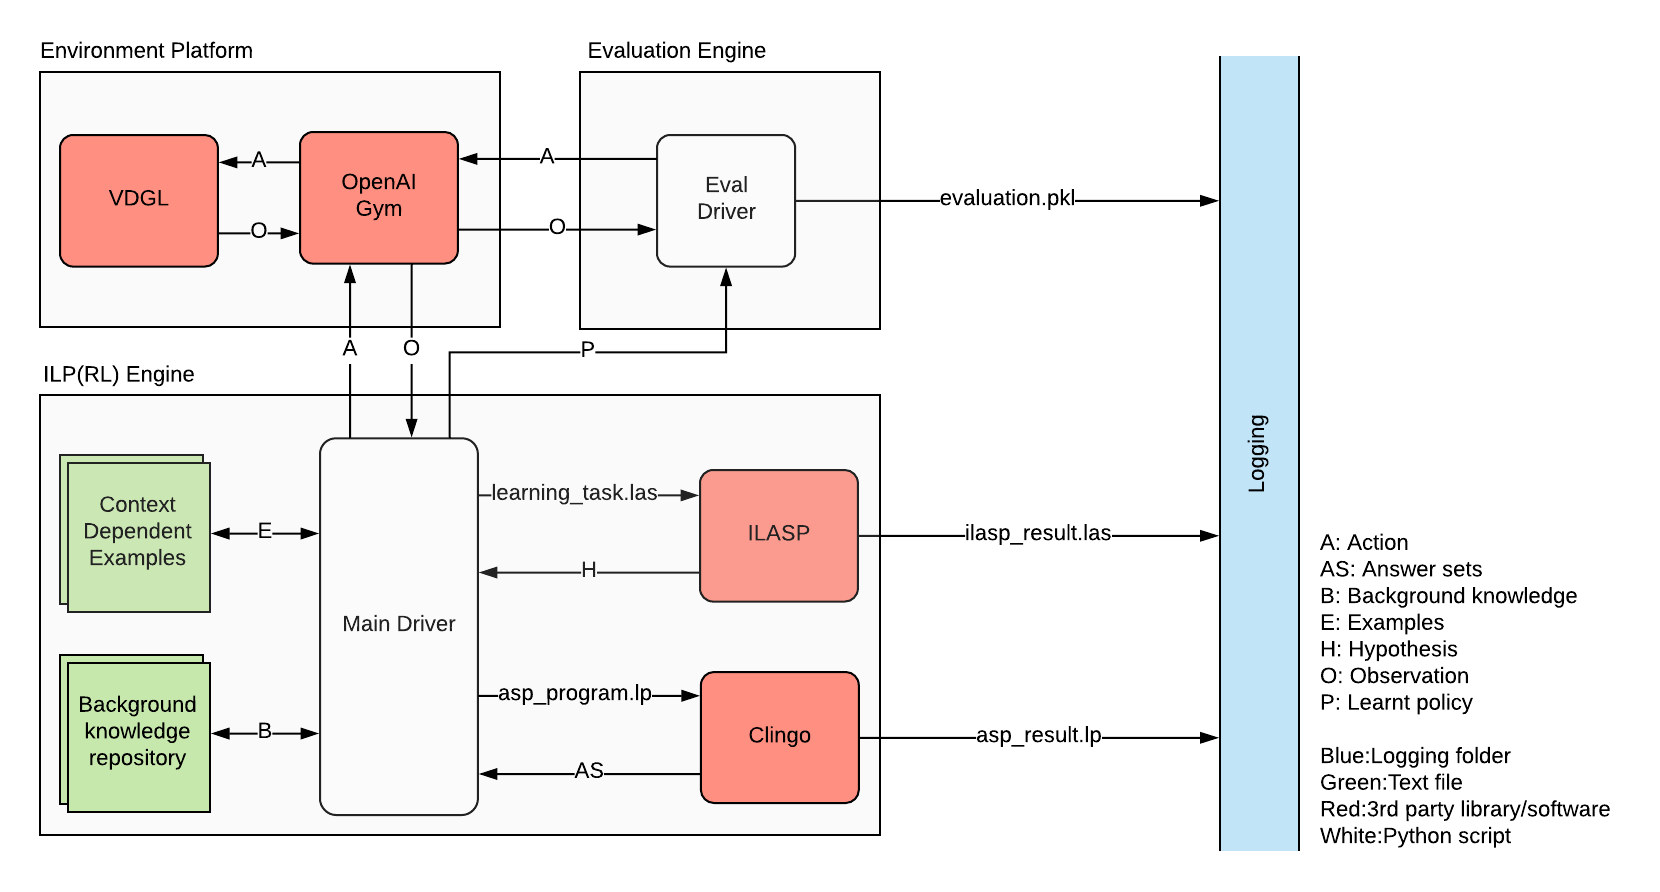
\includegraphics[width=1.0\textwidth]{./figures/ILPRL_dataflow}
\caption{Data flow diagram for ILP(RL) Engine, Environment and Evaluation components}
\label{fig:dataflow}
\end{figure}
We divide our implementation of the design outline into three separate software components: ILP(RL) Engine, Environment Platform and Evaluation Engine. The overview of our software implementation is shown in the data flow diagram in Figure \ref{fig:dataflow}. We describe each components of the implementation in the following sections.

\section{ILP(RL) Engine}
ILP(RL) Engine is our main framework explained in Chapter \ref{framework}. The main driver is written in Python and acts as an interface with different third-party libraries and software. 
\begin{itemize}
    \item create a learning task
\end{itemize}
The two main job of the driver is to execute inductive learning with ILASP, planning with ASP and the interaction with the environment platform provided by VGDL with OpenAI interface.
All of them are communicated through the main driver written in Python. 
In the following section, we explain each component of ILP(RL) in details.

\section{Inductive Learning with ILASP}
We use ILASP2i, an inductive learning system developed in \ref{Law2016b}.
ILASP2i is an iterative version of ILASP2, and is designed to scale with the numbers of examples. 
ILASP2i also introduces the use of context dependent examples.
The latest ILASP available is ILASP3, which is designed to work on a noisy examples. Our context dependent examples do not contain noise since they are all true state transition that the agent has experienced, and therefore ILASP2i was sufficient for our implementation.
which is discussed in Section XX. 
Although ILASP2i is designed to work with a large number of examples, inductive learning part is the bottleneck of our framework in terms of computational time. 
We did a number of optimisation in order to mitigate this. 

The first optimisation is the frequency of running ILASP. 
As already described in Definition \ref{def:ILASP_run}, ILASP is ran only if the current hypothesis does not cover all the examples accumulated so far.
Because of this, inductive learning takes place at the very early stage of learning, which is highlighted in the experiments in Chapter XX. 

The next optimisation is through the command line. 
ILASP2i has a number of options, and we explain each option using the actual command we use to run ILASP

% \begin{minted}[]
% ILASP --version=2i FILENAME.las -ml=8 -nc --clingo5 
% \end{minted}

\begin{lstlisting}[]
    ILASP --version=2i FILENAME.las -ml=8 -nc --clingo5 
    --clingo "clingo5 --opt-strat=usc,stratify" 
    --cached-ref=PATH --max-rule-length=8
\end{lstlisting}

where,
\begin{itemize}
\item \textsf{--version=2i} specifies that we use ILASP2i.
\item \textsf{--ml=8} specified the maximum numbers of body that each rule can have. The default length is 3.
\item \textsf{--nc} means no constrains, and omits constrains from the search space. Since our target hypothesis is not a constraint, this option reduces the search space.
\item \textsf{--clingo5} generates Clingo 5 programs, which is faster, instead of Clingo 4.3.
\item \textsf{--clingo "clingo5 --opt-strat=usc,stratify"} specifies Clingo executable with the specified options. 
\textsf{usc, stratify} is unsatisfiable-core base optimisation with stratification using Gringo \cite{gringo}, a core XXX introduced in gringo version 3. REFERENCE.
\item \textsf{--cached-ref=PATH} enables the iterative mode, and keeps the output of the relevant example to a specified path, and start the learning from where it left before rather than going though all the examples.
\item \textsf{--max-rule-length=8} The default maximum number is 5.
\end{itemize}

Last optimisation is specifying search space.

Complexity. 

TODO the number of search space XX. 

\section{Planning with ASP}
Planning is computed using Clingo 5.

\begin{lstlisting}[]
    clingo5 --opt-strat=usc,stratify -n 0 FILENAME.lp
    --opt-mode=opt --outf=2
\end{lstlisting}

\begin{itemize}
\item \textsf{--clingo "clingo5 --opt-strat=usc,stratify"} specifies clingo executable with the specified options. 
\textsf{usc, stratify} is unsatisfiable-core base optimisation with stratification using Gringo \cite{gringo}, a core XXX introduced in gringo version 3. REFERENCE.
\item \textsf{-n 0} -n is an abbreviation of \textsf{models} to specify the maximum number of answer sets to be computed. \textsf{-n 0} means to compute all answer sets.
\item \textsf{--opt-mode=opt} computes optimal answer sets
\item \textsf{--outf=2} makes the output in JSON\footnote{http://json.org/} format
\end{itemize}

\section{Environment Platform}
\subsection{The Video Game Definition Language (VGDL)}

\begin{figure}[!ht!b]
\centering
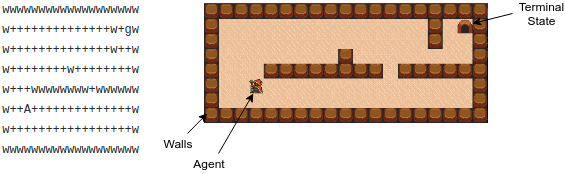
\includegraphics[width=1\textwidth]{./figures/env_sample}
\caption{Map sketch of a VGDL game (left) and it's high-level representation (right)} 
\label{VGDL_sample}
\end{figure}

We use the Video Game Definition Language (VGDL), which is a high-level description language for 2D video games providing a platform for computational intelligence research (\cite{Schaul2013}).
The VGDL allows users to easily craft their own environments, 
which makes us possible to do various experiments without relying on a default environment.

The base game we used to implement ILP(RL) is shown in Figure\ref{VGDL_sample}.
The map sketch is a plain text file and is easy to modify the configuration of the game.

\lstinputlisting[
    caption  = {VGDL description of a maze game},
    label = {list:vgdl}
]{vgdl.pl}

The behaviours of the game can be specified using VGDL as shown in \ref{list:vgdl}. 
All objects in the games can be described as a sprite in the \textit{SpriteSet}, where users can define the objects' properties.
\textit{InteractionSet} specify the effects of objects when two objects interact in the game.
\textit{TerminationSet} specify the conditions for ending the game.
The representation of each object can be specified in \textit{LevelMapping} and allows users to customise an original map.

We use PyVGDL\footnote{https://github.com/schaul/py-vgdl/}, which is a high-level VGDL on top of pygame\footnote{https://www.pygame.org}, 
a Python modules designed for writing video games.

\subsection{OpenAI Gym}
The VGDL platform provides an interface with OpenAI Gym (\cite{Brockman2016}), a commonly used benchmark platform for RL research.
The communication between VGDL environment and an agent, is through OpenAI Gym interface. 
\ref{list:openai} shows the functions provided by OpenAI Gym as well as the simple implementation for RL. 

In this report, an agent receives a reward of -1 for any state except the terminal state, and receives reward of +10 for the terminal state, or the goal.

% In all experiments, the agent receives -1 in any states except the goal state, where it gains a reward of 10.
% Once the agent reaches the goal, or termination state, that episode is finished and the agent start the next episode from the starting point.

\lstinputlisting[
  language = Python,
  caption  = {OpenAI gym interface},
  label = {list:openai}
]{openai.py}

\begin{itemize}
\item \textsf{env.reset()} resets the game and the agent starts from the starting position. We call it when the agent starts a new episode.
\item \textsf{env.step(action)} returns an observation of taking an action, which include the state location of the agent in terms of x and y coordinates, reward of the state, an boolean value indicating whether the agent reaches an terminal state.
The action is chosen by an RL algorithm of your choice. In the case of ILP(RL), action is chosen by the ASP planning or random exploration strategy between 0 and 3.
\item \textsf{env.render()} renders one frame of the environment to visualise the movement of the agent in pygame.
\end{itemize}

% \section{The Main Driver}
% All of the above are connected in Python script.

% The main roles of the driver is handling the communications between an environment and an agent as well as the communications within the agent.

% \begin{description}
% \item[Communication between an environment and an agent]

% When an agent takes an action in a VDGL game environment, 
% the output of the environment is returned by OpenAI gym environment, which is of the form:

% This works the same for any RL algorithms when using OpenAI gym environment. 

% subprocess

% \item[Communication within the agent]

% \end{description}
